\usepackage{titlesec}
\usepackage[ngerman]{babel}
\usepackage[a4paper, left=3cm, right=3cm, top=2cm, bottom=2cm]{geometry}
\usepackage{fouriernc}
\usepackage{titlesec}
\usepackage{keystroke}
\usepackage{csquotes}
\usepackage[ngerman]{babel}
\usepackage[dvipsnames]{xcolor}
\usepackage{graphicx} 
\usepackage{microtype}
\usepackage{float}
\usepackage{parskip}
\usepackage{amsmath}
\usepackage{hyperref}
\usepackage{enumitem}
\usepackage{dsfont}
\usepackage{algorithm}
\usepackage{float}
\usepackage[noend]{algpseudocode}
\usepackage{menukeys}
\usepackage{subfigure}
\usepackage{wrapfig}
\usepackage[onehalfspacing]{setspace}

\newcommand{\makeTitleAndTable}{
    \begin{titlepage}
        \centering
        \vspace*{1.5cm}
        {\Huge Einfacher SPH Flüssigkeitssimulator mit beschleunigter Nachbarschaftssuche\par}
        \vspace{1cm}
        {\LARGE Thierry Meiers\par}
        {\Large Bachelor Projekt\par}
        \begin{figure}[H]
            \centering
            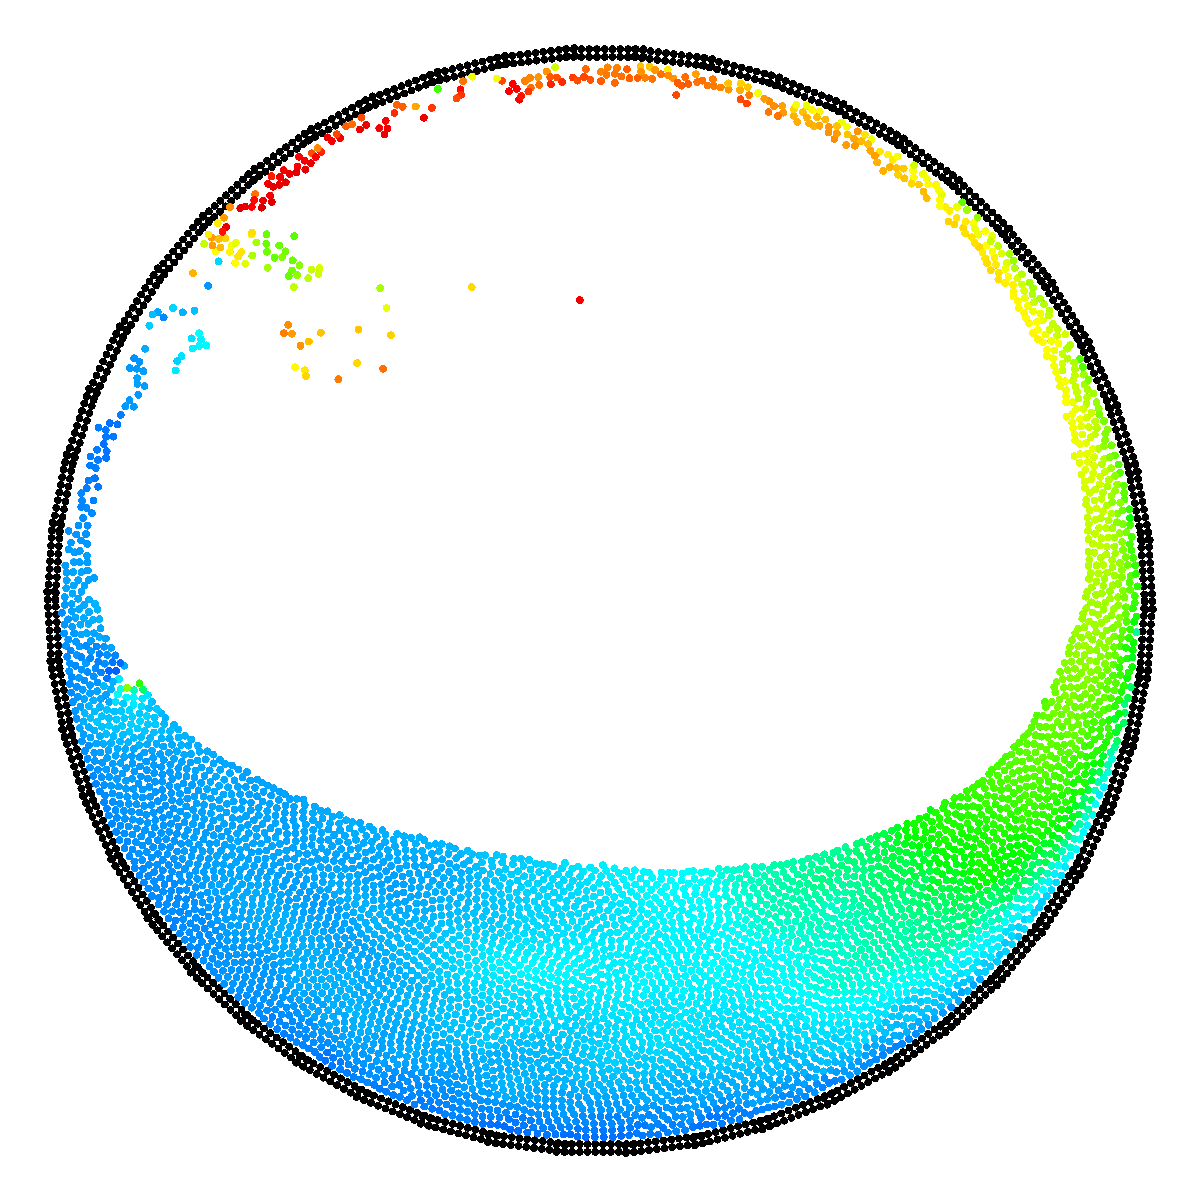
\includegraphics[width=.7\textwidth]{graphics/FirstPage.png}
        \end{figure}
        \vspace{0.5cm}
        {\large Albert-Ludwigs-Universität Freiburg\\Technische Fakultät\\Graphische Datenverarbeitung\par}
        \vfill
        {\large \today \par}
    \end{titlepage}
    \pagenumbering{gobble}
    \tableofcontents
    \clearpage
    \pagenumbering{arabic}
}
